\chapter{jInfer}
\label{appendix-jInfer}

This appendix describes shortly yet comprehensively \textbf{jInfer} - the Java framework for XML schema inference, in which the algorithms described in this work were implemented. Please see project web \cite{jinferweb} for complete information, documentation and download options.

jInfer was developed between 2009 and 2011 at the Charles University in Prague as a Software Project by team consisting of Michal Klempa, Mário Mikula, Ro\-bert Sme\-ta\-na, Michal Švirec and Matej Vitásek. The main idea was to create a structure in which all aspects of XML schema inference can be easily implemented and evaluated. The goal was achieved: the SW project was successfuly defended when jInfer was inferring DTD and XSD schemas based on XML documents, old DTD and XSD schemas and XPath queries. Since then, Michal Klempa has successfuly defended his own thesis improving on the grammar simplification process (see below), Michal Švirec has extended the framework with capabilities to detect and repair functional dependencies violation (see \cite{sviro}) and defended his thesis as well. This thesis is the third one based on this framework, and Mário Mikula's is on its way, too.

To the best of our knowledge, at the time of writing this thesis is jInfer the only public, open source and actually working solution for XML schema inference-related tasks.

At heart of jInfer inference process is a modular system provided by NetBeans Platform allowing to define services (interfaces), implement them in any number of ways and then let the user choose which implementation to use. Most importantly, the whole process consists of 3 consecutive steps (see \ref{image-inference-process}), responsibility of 3 different services - interchangeable modules.

\begin{figure}
  \caption{Inference Process in jInfer}
  \vspace{10pt}
  \label{image-inference-process}
  \centering
    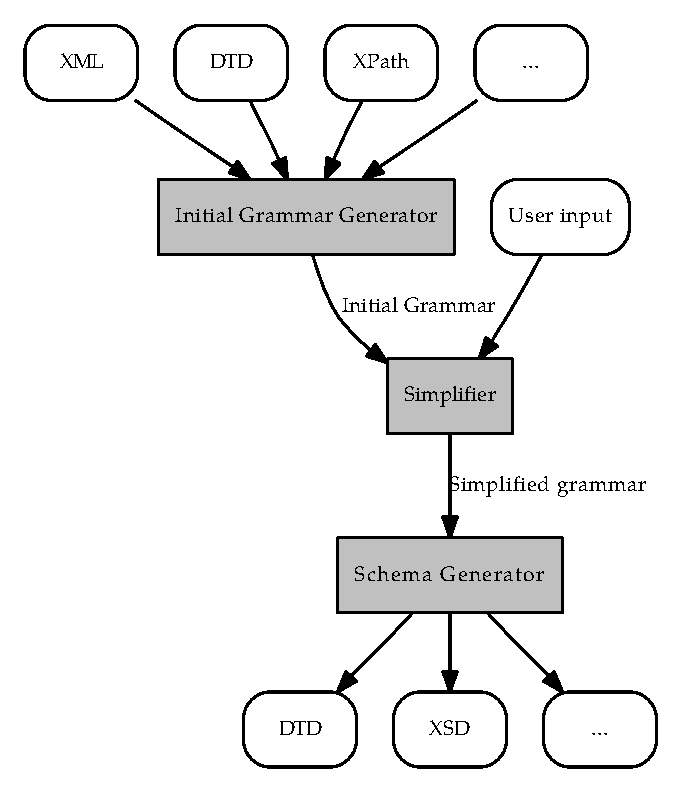
\includegraphics[width=0.5\textwidth]{images/inference-process}
\end{figure}

The responsibility of the first module, the \jmodule{Initial Grammar Generator}, is~to~parse all input files (documents, schemas and queries) and create a so-called \textit{initial grammar} (IG). \nomenclature{IG}{Initial Grammar}
This is the representation in which will the structure live until it is used to create the final product - the schema. As the name suggests, IG is a grammar - an \textit{extended context-free grammar}, to be more precise (see \cite{extendedcfg}). As such, its left-hand side is an element, its right-hand side is a regular expression representing its content model. IG is used to create the AM model used in this thesis, too. jInfer contains one such module, the \jmodule{BasicIGG}, which is described in detail in \cite{basiciggdoc}.

After leaving the \jmodule{Initial Grammar Generator}, the IG needs to be made more general, shortened, \textit{simplified}. This is the responsibility of an aptly named module, the \jmodule{Simplifier}. To get the full idea about how this can be done it~would be probably best to read Michal Klempa's thesis \cite{anti}, which describes this in great detail. Whatever happens, there is simplified grammar on~the exit of \jmodule{Simplifier}, ready to be processed by...

The last module, \jmodule{Schema Generator} takes the simplified grammar and creates the resulting schema from it. This process is not too interesting, but anyone wishing to find out all about it is invited to read the documentation to the two \jmodule{Schema Generator}s bundled with jInfer - the BasicDTD and BasicXSD modules.
